\documentclass[../root]{subfiles}
\graphicspath{{_images/}{../_images/}}


\begin{document}

    \chapter{Avoiding the ask: A field experiment on altruism, empathy, and charitable giving}

    \begin{shortsummary}
        \begin{itemize}
            \item \authoryear{Andreoni2017}
            \item \RQ{向社会的行動の勧誘を避ける行動は利他的な人が自身の感情をコントロールした結果で生じているのか?}
            \item \answer{スーパーマーケットで行ったファンドレイジング運動のフィールド実験}
            \item \result{罪悪感を刺激するような方法を用いると、募金活動のパフォーマンスが挙がる一方で募金活動の場所に向かわないような人も現れた。これは勧誘員に寄付しないと回答することで生じる罪悪感を回避しているからと考えられる}
        \end{itemize}
    \end{shortsummary}

    \section{Research Question}

    \begin{itemize}
        \item warm glowは向社会的行動自体に効用を得るという概念であり、これは様々な要素を含む
        \begin{itemize}
            \item Social concernsは主な要素の一つであり、(1) 自分が社会規範に沿った人間であるという自己のイメージを保ちたい動機や(2) レシピエントが形成する良い社会的イメージを維持したいという動機などがある
        \end{itemize}
        \item また、\textbf{向社会的行動を避けられる機会が提供されるとき、向社会的行動をしない選択をする人が存在する}ことも分かっている
        \item このfindingは、寄付行為で効用を得られないという帰結よりもむしろ、\textbf{利他的な個人が非向社会的な行動をとることで感じる罪の意識を自覚したうえでそれを軽減するためにとった行動 (Sophisticated altruist)}と考える方が自然であると主張している
        \item 利己的な人はavoidingすることで罪悪感の不効用を得ないはずなので、avoidingをあえてとるような行動は考えにくい
        \item フィールド実験にて、\textbf{向社会的行動の要請を避ける行動は利他的な人が自身の感情をコントロールするために生じているのかどうか}を分析した
    \end{itemize}

    \section{Experimental Design}

    \subsection{Outline}

    \begin{itemize}
        \item Salvation Red Kettle Campaignとの共同研究で、ボストン地区のスーパーマーケットで実施
        \item スーパーマーケットの出入り口で募金活動をする
    \end{itemize}

    \begin{figure}[h]
        \centering
        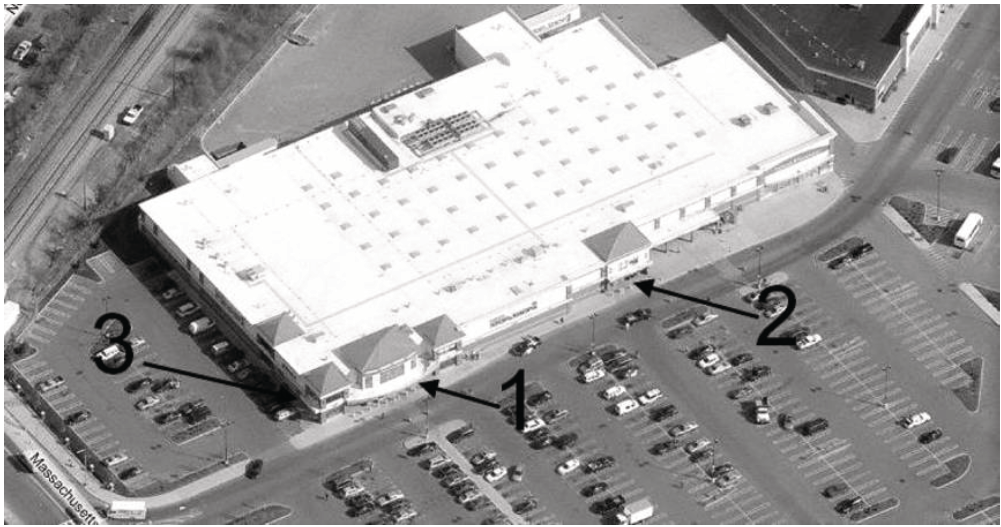
\includegraphics[width = 0.8\linewidth]{0821kato/fig1_1.png}
        \caption{実験場所であるスーパーマーケットの外観}
        \label{}
    \end{figure}

    \begin{itemize}
        \item 2-by-2 between treatment
        \begin{enumerate}
            \item 勧誘員はベルを鳴らすだけ(Opp)か、それに加えて「寄付をしてください」と声をかける(Ask)
            \item 勧誘員は出入口1だけにいる(Opp1, Ask1)か、出入口1と2にいる(Opp 1\&2, Ask 1\&2)
        \end{enumerate}
        \item データ
        \begin{itemize}
            \item 各勧誘員が寄付者の数をカウントしたデータ
            \item RAを雇い、出入口1と2から出た人と入った人をカウントする
        \end{itemize}
        \item 結果の概要
        \begin{itemize}
            \item Oppトリートメントでは、客の出入りに大きな変化はなかった
            \item Opp1\&2トリートメントの寄付者数は、Opp1の2倍になった
            \item Ask1トリートメントの寄付者数と寄付総額は、Opp1と比べて45-69\%増加した
            \item Ask1トリートメントでは、1/3の客が勧誘員が立っていないドアを選択するようになった
        \end{itemize}
    \end{itemize}


    \subsection{Details}

    \begin{figure}[h]
        \centering
        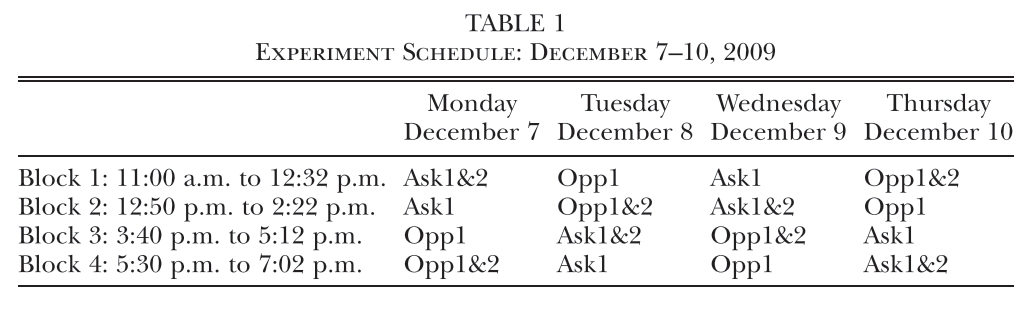
\includegraphics[width = 0.8\linewidth]{0821kato/fig2_1.png}
        \caption{実験スケジュール}
        \label{}
    \end{figure}

    
    \begin{itemize}
        \item 各ブロックは92分で構成されており、23分のセッションごとにデータを記録している(1ブロック = 4セッション)
        \begin{itemize}
            \item トラフィックデータはブロック単位でとれたが、寄付データはセッション単位でとれた
        \end{itemize}
        \item 実験スケジュールは以下の点を考慮して決定されている
        \begin{itemize}
            \item daily balance: 曜日などの固定効果を排除する
            \item time balance: 繁忙時間などの固定効果を排除する
            \item 入退店両方でAskかOppのトリートメントを受けるようにしている(しかし、Doorトリートメントは異なる可能性が十分にある)
        \end{itemize}
        \item 実験の後日(2013年7月)に改めて客の移動についてデータ採取した。これは以下の点を考慮するためである
        \begin{itemize}
            \item 曜日×時間の固定効果が存在するかどうかを確かめるため
            \item 小サンプル(最大でN=64)によって統計的推論を誤った方向に導く可能性があるので、それを確かめるため
        \end{itemize}
        \item 実験実施時、ドア3のトラフィックデータを採取していなかったので、ドア1と2のデータから推論するしかない
    \end{itemize}

    \section{Theoretical Framework}

    \subsection{Settings and Notations}

    \begin{itemize}
        \item 出入口の選択と勧誘員が立っている出入口を通過したときの2時点間の意思決定とみなす
        \begin{itemize}
            \item 出入口選択時は、勧誘員からの声掛けとかがないため、感情に従わない意思決定をする(planner)
            \item 出入口通過時は、勧誘員からの声掛けとかがあるため、感情に従う意思決定をする(short-run self)
        \end{itemize}
        \item $u$: 勧誘員が立っている出入口に向かい、最適な寄付gをするときの効用
        \item $v$: 勧誘員が立っていない出入口を使い、寄付をしないときの効用
        \begin{itemize}
            \item お金を節約するベネフィットと罪悪感の心理的コストがある
        \end{itemize}
        \item $g_0$: 意思決定時(出入口の選択時)に考えていた最適な寄付額
        \begin{itemize}
            \item 勧誘員に直接を声をかけるなどによって、$g_0$が最適とならないケースがある($g_0$では罪悪感を得てしまう)。その場合、$g > g_0$となる
        \end{itemize}
        \item $c>0$: 一番近い出入口から他の出入口に変えるときの移動コスト
    \end{itemize}

    \subsection{Behavior Type}

    \begin{itemize}
        \item 寄付をする人は2つのタイプがある
        \begin{itemize}
            \item \textit{passive givers} ($u > v - c$ \& $g > 0$):一番最適なドアを利用して寄付をする人
            \item \textit{seeking givers} ($u - c > v$ \& $g > 0$):一番最適なドアからあえて勧誘員のいるドアに変えて寄付をする人
        \end{itemize}
        \item 寄付をしない人は3つのタイプがある
        \begin{itemize}
            \item \textit{passive non-givers} ($u > v - c$ \& $g = 0$):一番最適なドアを利用して寄付しない人
            \item \textit{giving avoiders} ($v - c > u$ \& $g > g0$):勧誘員がいるドアを利用すると罪悪感を感じるのでplannerが最適と考える寄付を増やすので、それを避けるように別の出入口を使う人
            \item \textit{saying no avoiders} ($v - c > u$ \& $g = g0 = 0$):plannerが寄付しないことを最適と考え、感情に左右されずにそれを実行できる人が、「寄付しない」と勧誘員に意思表示することで感じる罪悪感を避けるように別の出入り口を使う
        \end{itemize}
    \end{itemize}

    \subsection{Corresponding to Experimental Variation}

    \begin{itemize}
        \item 勧誘員が立っている出入口を2つに増やす:移動コストcを高める
        \item Verbal ask:少額の寄付や「寄付しない」という意思表示に伴う罪悪感を高める
    \end{itemize}


    \section{Result}

    \subsection{Fundraising Performance}

    \begin{figure}[t]
        \centering
        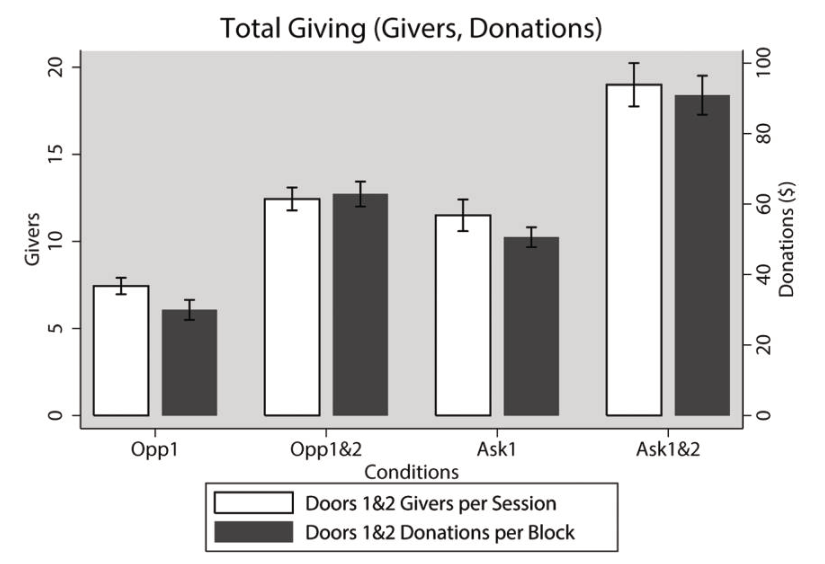
\includegraphics[width = .8\linewidth]{0821kato/fig3_1.png}
        \caption{Total Giving and Total Givers}
        \label{}
    \end{figure}

    \begin{figure}[t]
        \centering
        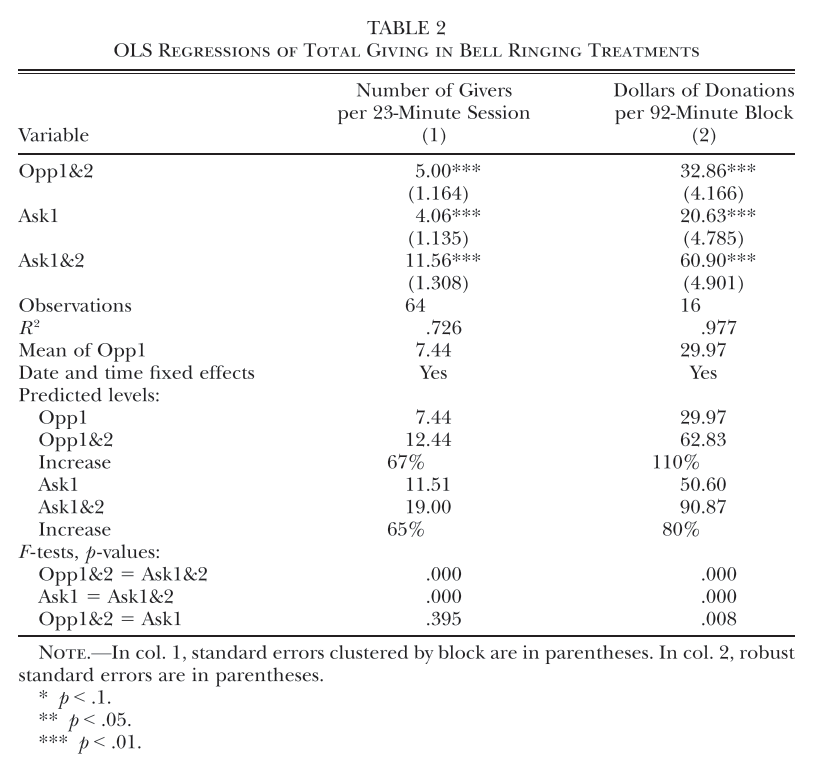
\includegraphics[width = .8\linewidth]{0821kato/fig4_1.png}
        \caption{Regression Results}
        \label{}
    \end{figure}

    \begin{itemize}
        \item verbal askを追加することで、寄付者と寄付額が増えた
        \begin{itemize}
            \item Opp1 vs Ask1:寄付者+55\%、寄付額+69\%
            \item Opp1\&2 vs Ask1\&2:寄付者+53\%、寄付額+45\%
        \end{itemize}
        \item 勧誘員を一人追加することで、寄付者と寄付額が増えた
        \begin{itemize}
            \item Opp1 vs Opp1\&2:寄付者+67\%、寄付額+110\%
            \item Ask1 vs Ask1\&2:寄付者+65\%、寄付額+80\%
        \end{itemize}
        \item フレームワークからpotential donor($g > 0$)は3タイプ:seeking givers, giving avoiders, passive givers
        \begin{itemize}
            \item 全員がpassive giversならば、2 door conditionのアウトカムは1 door conditionの2倍になるはず$\to$\textit{説明できない}
            \item seeking giversがdominateしているならば、ドアコンディションがアウトカムに影響を与えることはない$\to$\textit{説明できない}
            \item giving avoidersがdominateしているならば、1ドアコンディションのアウトカムが極端に少ないはず$\to$\textit{説明できない}
        \end{itemize}
    \end{itemize}

    \subsection{Traffic Data}

    \begin{figure}[t]
        \centering
        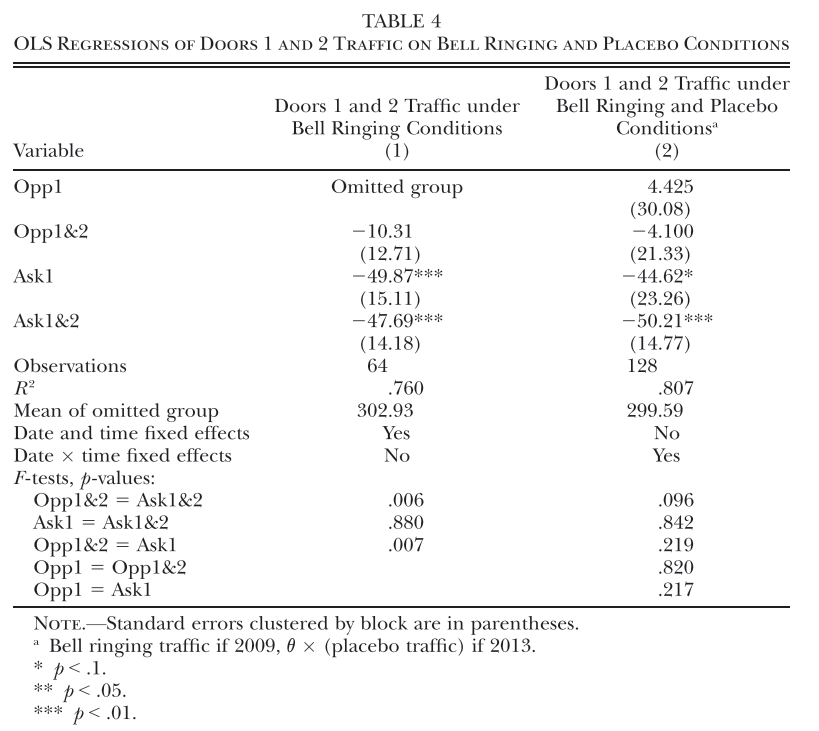
\includegraphics[width=.8\linewidth]{0821kato/fig5_1.png}
        \caption{Regression Results}
        \label{}
    \end{figure}

    \begin{itemize}
        \item Ask conditionのもとでは、ドア1と2を利用する客がそれぞれ16.5\%と15.7\%減少した
        \begin{itemize}
            \item 解釈1:そもそもAsk conditionをアサインした時間帯の利用客数が少ない
            \item 解釈2:ドア3を利用するようになった可能性がある
        \end{itemize}
        \item 勧誘員を増やすこと(Ask1\&2とOpp1\&2)は利用客の減少につながらない
        \begin{itemize}
            \item ドア2が最も近い人が寄付勧誘を避けるためにドア3を避けるためには、コストが大きすぎるので、giving avoiderがoptimal strategyではないのかもしれない。
        \end{itemize}
    \end{itemize}

    \begin{figure}[t]
        \centering
        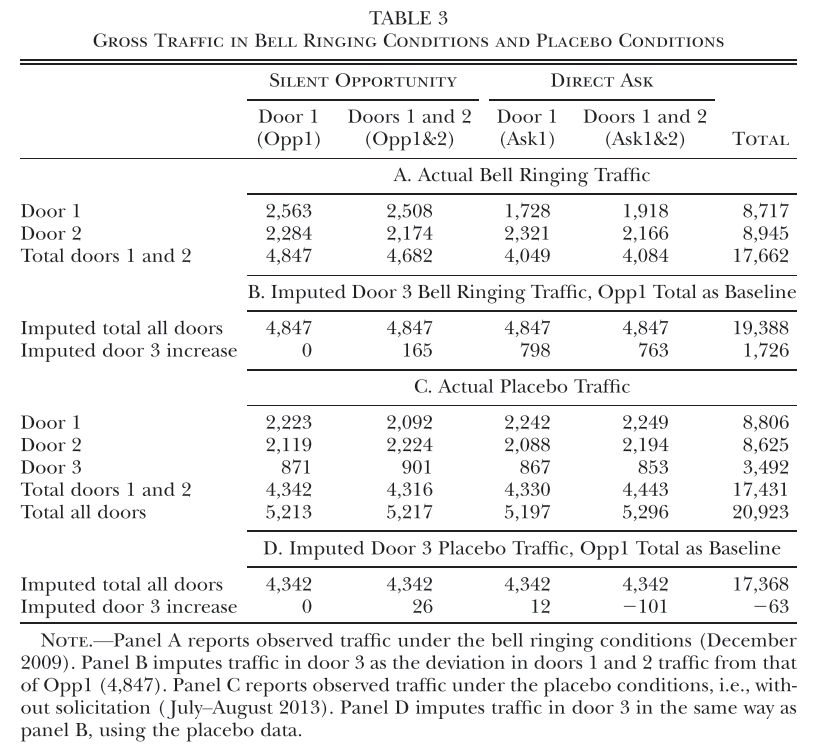
\includegraphics[width=.8\linewidth]{0821kato/fig6_1.png}
        \caption{Gross Traffic across Treatments}
        \label{}
    \end{figure}

    \begin{itemize}
        \item 解釈1の可能性を排除するために、2013年に同じ時間帯のトラフィックデータを採取してOpp1の利用客数との差分を調べた。結果、実験で観察された減少分を説明できるほどトリートメント間のトラフィックに差がなかった(パネルBとD)
        \item 頑健性の確認のために、プラセボデータを加えた回帰分析をやっているが、結果に大きな変化はない。
        \item ドア1とドア2に分けて、同じ分析をしているが、やはり結果は変わらない
    \end{itemize}

    \subsection{Inference of Behavior Type from Door1 Performance}

    \begin{figure}[t]
        \centering
        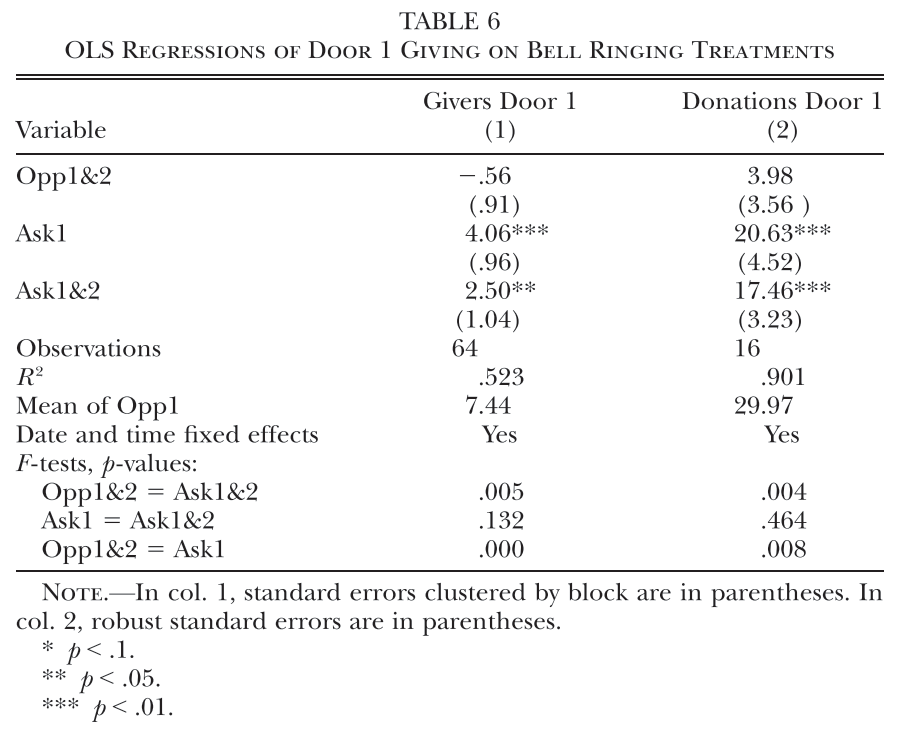
\includegraphics[width = .8\linewidth]{0821kato/fig7_1.png}
        \caption{Regression on Fundraising Performance at Door 1}
        \label{}
    \end{figure}

    \begin{itemize}
        \item silent opportunity conditionは罪悪感を喚起する可能性が低いので、このトリートメントのもとでgiving avoiderはいない
        \begin{itemize}
            \item 可能性1:passive giversがdominateしているならば、door condition間で結果に変化がないはず
            \item 可能性2:seeking giversがdominateしているならば、one door conditionの寄付者数はtwo doorsの2倍になるはず
        \end{itemize}
        \item Opp1とOpp1\&2の間で結果に差がないので、\textbf{silent conditionではpassive giverがdominateしている}可能性がある
        \item Verbal conditionは罪悪感を喚起しやすいので、avoiderの存在を考慮する必要がある
        \begin{itemize}
            \item Ask1とAsk1\&2の結果にavoiderの数が含まれる(とくにAsk1\&2)ので、Ask1とAsk1\&2の比較がseeking giversの存在を示すには不十分である
            \item avoiderとseekerを区別して識別することは不可能
        \end{itemize}
        \item Verbal conditionのもとで寄付者のタイプの割合を調べるために、total donationsに焦点を当てる
        \begin{itemize}
            \item seekerがdominateしているならば、Ask1のアウトカムはAsk1\&2より多くなるはず
            \item avoiderがdominateしているならば、Ask1のアウトカムはAsk1\&2より少なくなるはず
            \item ask1とAsk1\&2の総寄付額に差がないということは、seekerとavoiderの比率がほぼ一緒であることで説明がつく
            \item Ask1の寄付額がAsk1\&2より若干多いことから、avoiderは要求を受けても寄付しないのかもしれない
            \begin{itemize}
                \item したがって、giving avoiderは\textbf{saying no avoider}である可能性が高い
            \end{itemize}
        \end{itemize}
    \end{itemize}

    \biblio

\end{document}